\documentclass[12pt]{article}

\usepackage{kpfonts} % change the fonts
\usepackage[portuguese]{babel}
\usepackage[margin=1in]{geometry} % change the margins of the page
\usepackage{hyperref} % allow to use hyperlink on websites and e-mails, for example
\usepackage[T1]{fontenc}
\usepackage{graphicx} % to import figures
\usepackage[export]{adjustbox}
\usepackage{booktabs} % to create tables
\usepackage{threeparttable} % to create nice tables with notes
\usepackage{arydshln} % allows for dashed lines on tables
\usepackage{placeins}
\usepackage{caption} % add note to figures
\usepackage{capt-of}
\usepackage{setspace} % change spacing
\usepackage{indentfirst}

\doublespacing
\setlength{\parskip}{0.75em}

\title{Real-Time Electricity Consumption and the Economic Impacts of COVID-19 in Brazil}
\author{Gabriel Richter de Almeida\footnote{FGV EPGE - Brazilian School of Economics and Finance. E-mail:\href{mailto:gabriel.richter@outlook.com}{gabriel.richter@outlook.com}}}
\date{\today}

\begin{document}
	
\section*{\normalsize Consumo de Eletricidade e os Impactos Econômicos do COVID-19 no Brasil \\	Gabriel Richter de Almeida (FGV EPGE) \\ \today}
	
Já não há dúvidas de que a pandemia do Coronavírus 2019 (COVID-19) produziu efeitos perversos sobre a atividade econômica brasileira. Dados recentes divulgados pelo Instituto Brasileiro de Geografia e Estatística (IBGE) sugerem que o Produto Interno Bruto (PIB) do Brasil desabou 11,4\% no 2º trimestre de 2020, relativamente ao mesmo trimestre de 2019. Com a gradual flexibilização das regras de isolamento social vigentes nos últimos meses, a expectativa é de que o pior já tenha ficado para trás, em que pese a tristeza deixada pelas mais de cem mil vidas humanas perdidas -- e assumindo-se que não haja um aumento expressivo do número de casos que torne necessária a implementação de novos lockdowns. No entanto, o ritmo de recuperação da atividade econômica ainda é objeto de discussão entre os economistas. Terá ela um formato de “Z”, “V”, “U”, “Nike”, “W”, ou “L”? A resposta para essa pergunta é importante, pois serve de norte para que o governo avalie e calibre políticas públicas de estímulo à economia, bem como para o Banco Central, na condução de sua política monetária.
	
Nesse contexto de incertezas, dados de alta-frequência podem ser utilizados como uma interessante ferramenta para medirmos a temperatura da economia. A vantagem é que esse tipo de informação fornece, em tempo real, uma fotografia do que as estatísticas oficiais só revelarão semanas à frente. Embora não sejam, de forma alguma, substitutos às estatísticas oficiais, esses dados alternativos vêm sido paulatinamente adotados ao redor do mundo. Por exemplo, pesquisadores do \href{https://opportunityinsights.org/}{\textit{Opportunity Insights}}, da Universidade de Harvard, acompanham diariamente a recuperação da economia norte-americana através de dados de compras de cartão de crédito e débito, folhas de pagamento e vagas de trabalho publicadas online. No \href{https://budgetmodel.wharton.upenn.edu/}{\textit{Penn Wharton Budget Model}}, formado por pesquisadores da Universidade da Pensilvânia, utiliza-se também dados de tráfego a estabelecimentos comerciais e de concentração de poluentes ligados à atividade industrial para se construir um ``rastreador'' do PIB americano, atualizado diariamente. \vspace{5pt}
	
\begin{figure}[!bp]
	\centering
	\caption{Consumo de Eletricidade vs. PIB -- Brasil, por Trimestre}
	\label{fig:figure1}
	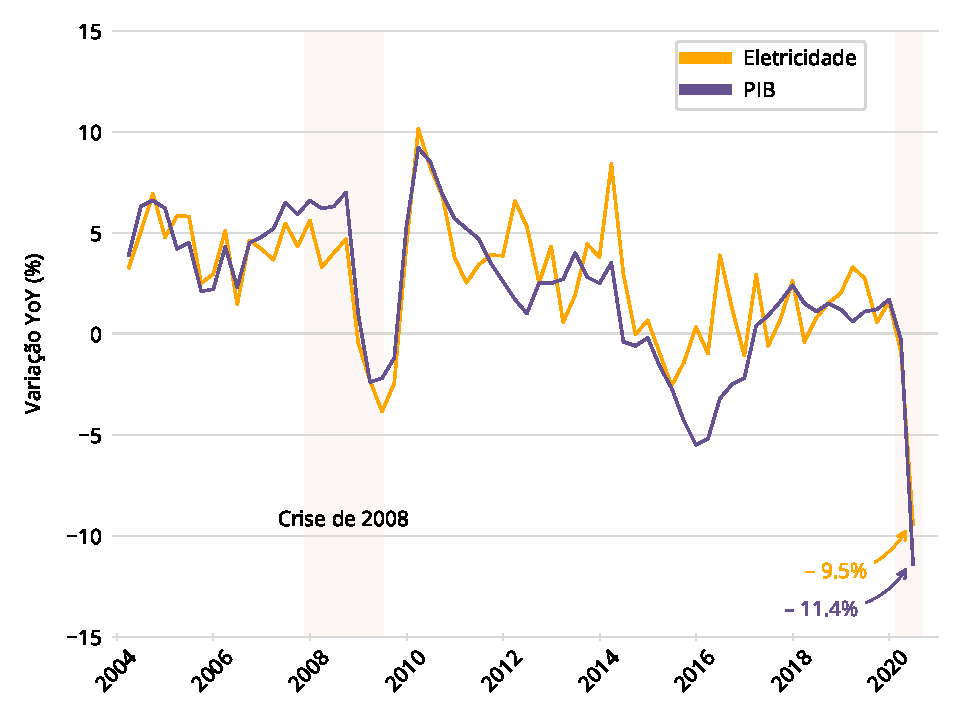
\includegraphics[width=\linewidth, keepaspectratio]{C:/Users/gabri/Desktop/electricity_rt/figures/historical_notitle.pdf}	
	\captionsetup{font={small}}
	\caption*{\textsuperscript{1} Fontes: IBGE e ONS.}
\end{figure}
	
Muitos dos dados utilizados por esses institutos de pesquisa são proprietários e obtidos através de empresas parceiras. No entanto, há uma informação de mais fácil acesso, disponível em tempo real, e que historicamente apresenta forte correlação com o nível de atividade econômica: o consumo de eletricidade. A intuição, que é bastante simples, é que quase toda atividade econômica utiliza energia como insumo. A Figura~{\ref{fig:figure1}} mostra que, nos últimos dezesseis anos, as taxas de crescimento trimestral (YoY) do PIB brasileiro e do consumo de eletricidade exibiram um comportamento muito semelhante -- lembrando, sempre, que correlação não implica em causalidade! Em particular, durante a crise financeira de 2008, ambas tiveram uma dinâmica de queda e recuperação parecida. Porém, enquanto as informações sobre o uso de energia eram conhecidas em tempo real, os dados oficiais do PIB só foram anunciados meses mais tarde. 

Agora, durante a pandemia do COVID-19, enquanto o consumo de eletricidade caiu 9,5\% no segundo trimestre de 2020, relativamente ao mesmo trimestre de 2019, o PIB caiu 11,4\%. É claro, não há garantia de que esse padrão continuará existindo no longo prazo. Afinal, transformações estruturais -- tais como a redução do peso de atividades intensivas em energia na composição do PIB, padrões de consumo mais sustentáveis, e ganhos de eficiência energética -- podem provocar um descolamento entre essas duas curvas. Para além disso, diferentemente de crises passadas, esta é uma crise de saúde pública e, portanto, apresenta particularidades que devem ser levadas em consideração. Por exemplo, muitos empregados foram obrigados a substituir o trabalho no escritório pelo regime de home office. Isso posto, se o nível de energia consumido ao se trabalhar de casa for semelhante ao que seria utilizado no escritório, então é plausível afirmar que a queda no consumo de eletricidade terá reflexos mais próximos àqueles sobre a atividade econômica. Por outro lado, caso o home office se traduza em maior eficiência no consumo de energia -- ou, talvez, um consumo inferior em virtude da expectativa de que contas de luz mais elevadas não serão reembolsadas pelo empregador, então a queda da atividade econômica poderá ser menor.

Em linha com um \href{https://home.uchicago.edu/~scicala/papers/real_time_EU/real_time_EU.pdf}{trabalho} desenvolvido pelo economista Steve Cicala, da Universidade de Tufts, criei um indicador que mede a variação diária do consumo de eletricidade no Brasil, em 2020, relativamente ao período pré-COVID -- que defini como sendo de 01 de janeiro a 29 de fevereiro de 2020, pouco antes da doença ter sido declarada uma pandemia pela Organização Mundial da Saúde (OMS), em 11 de março de 2020. Os dados de uso de eletricidade utilizados como insumo para a construção desse indicador foram obtidos através do Operador Nacional do Sistema Elétrico (ONS) e são divulgados em tempo real. Eles representam cerca de 99\% de toda a eletricidade consumida no país por clientes comerciais, industriais e residenciais. Essas informações estão disponíveis para quatro subsistemas, segundo uma classificação estabelecida pela ONS. São eles os subsistemas Norte, Nordeste, Sudeste/Centro-Oeste e Sul. Praticamente todos os estados pertencem ao subsistema homônimo à região brasileira da qual fazem parte, com exceção do estado do Maranhão, que faz parte do subsistema Norte, dos estados do Acre e Rondônia, que fazem parte do subsistema Sudeste/Centro-Oeste, e do estado de Roraima, que não é incluído em subsistema algum e que, portanto, é excluído da análise. Adicionalmente, utilizei dados de satélite e radar para obter a temperatura, por hora, de todos os municípios brasileiros; e dados de feriados nacionais, disponibilizados pela Associação Brasileira das Entidades dos Mercados Financeiro e de Capitais (ANBIMA).

Não surpreendentemente, o consumo de eletricidade possui padrões sazonais. Ele é (1) superior durante o horário de trabalho, vis-à-vis ao período da madrugada e noite; (2) maior nos dias de semana, relativamente aos finais de semana; (3) inferior durante feriados nacionais; (4) maior no verão do que no inverno; (5) e superior quando temperaturas mais elevadas estimulam o uso de aparelhos de ar-condicionado. Portanto, de forma a permitir a comparação entre diferentes momentos no tempo, os dados de consumo foram dessazonalizados. Adicionalmente, os valores do indicador são normalizados para terem média zero entre 01 de janeiro e 29 de fevereiro de 2020. A normalização é importante, pois nos permite medir o quanto o consumo de eletricidade variou relativamente ao período que antecedeu a pandemia. 

Um indicador distinto (Figuras~{\ref{fig:figure2}} a ~{\ref{fig:figure5}}) foi criado para cada subsistema. A média ponderada desses indicadores, por sua vez, deu origem a um indicador nacional (Figura~{\ref{fig:figure6}}), onde para cada subsistema foi atribuído um peso proporcional à sua fração no consumo total do país entre 2016 e 2019. \vspace{5pt}

\begin{table}[!htp]
	\centering
	\caption{Indicador de Consumo de Eletricidade -- Variação Mensal em 2020}
	\label{tab:table1}
	\begin{threeparttable}[!hp]
		\begin{tabular}{lrrrrrr}
			\\[-0.75em] \toprule \\[-1em]
			{} &  Março &  Abril &  Maio &  Junho &  Julho &  Agosto \\
			\midrule \\[-1em]
			Nordeste             &       -4,29\% &      -11,81\% &      -10,95\% &       -7,35\% &       -4,41\% &       -4,86\% \\ \\[-1em]
			Norte                 &       -4,88\% &      -11,11\% &       -8,07\% &       -3,55\% &       -1,49\% &        1,85\% \\ \\[-1em]
			Sudeste/Centro-Oeste &       -2,43\% &      -11,25\% &       -8,58\% &       -5,05\% &       -1,54\% &        0,63\% \\ \\[-1em]
			Sul                 &        1,08\% &      -10,82\% &       -6,41\% &       -9,13\% &       -7,08\% &       -5,83\% \\ \\[-1em] \hdashline[2pt/3pt] \\[-0.75em]
			Brasil                &       -2,33\% &      -11,26\% &       -8,55\% &       -6,01\% &       -2,97\% &       -1,29\% \\ \\[-1em]
			\bottomrule \\[-0.75em]
		\end{tabular}
		\begin{tablenotes}
			\item[1] \small Valores normalizados para terem média zero entre 01 de janeiro e 29 de fevereiro de 2020. Portanto, devem ser interpretados relativamente ao período pré-COVID.
			\item[2] \small Fontes: ONS e autor.
		\end{tablenotes}
	\end{threeparttable}
\end{table} 

Os resultados da Tabela~{\ref{tab:table1}} sugerem que o consumo em março caiu em quase todos os subsistemas, com exceção do subsistema Sul, onde cresceu 1,08\% relativamente ao período pré-pandemia. Em abril, o uso de eletricidade despencou aproximadamente 11\% em todo o país, coincidindo com um momento no qual diretrizes de distanciamento social foram reforçadas e políticas de lockdown ampliadas nacionalmente, fechando aeroportos, comércios, fábricas e escritórios. 

Nos subsistemas Nordeste (Figura~{\ref{fig:figure2}}) e Sul (Figura~{\ref{fig:figure5}}), a retomada aos níveis pré-pandemia tem se mostrado mais lenta. O primeiro exibiu uma retomada significativa entre os meses de maio e julho, sucedida por uma piora marginal no mês de agosto. O consumo de eletricidade no subsistema Sul, por sua vez, apresentou uma melhora substancial no mês de maio, vis-à-vis à queda expressiva do mês de abril. No entanto, voltou a cair no mês de junho -- o oposto do que se observou nas demais regiões do país, para então tornar a crescer novamente nos meses de julho e agosto. Por outro lado, nos subsistemas Norte (Figura~{\ref{fig:figure3}}) e Sudeste/Centro-Oeste (Figura~{\ref{fig:figure4}}) -- neste último, onde se concentra mais da metade do consumo de eletricidade em todo o país, o uso de energia já retornou aos níveis pré-COVID. 

Por fim, o que se observa a nível nacional (Figura~{\ref{fig:figure6}}) é uma recuperação consistente desde a metade de abril. Se a relação entre o consumo de eletricidade e a atividade econômica observada nos últimos dezesseis anos continuar valendo, então há evidência de que recuperação do PIB brasileiro poderá ser bastante rápida, tal qual foi a sua queda. A confirmar. \vspace{5pt}

\begin{figure}[!htb]
	\centering
	\caption{Indicador de Consumo de Eletricidade -- Nordeste}
	\label{fig:figure2}
	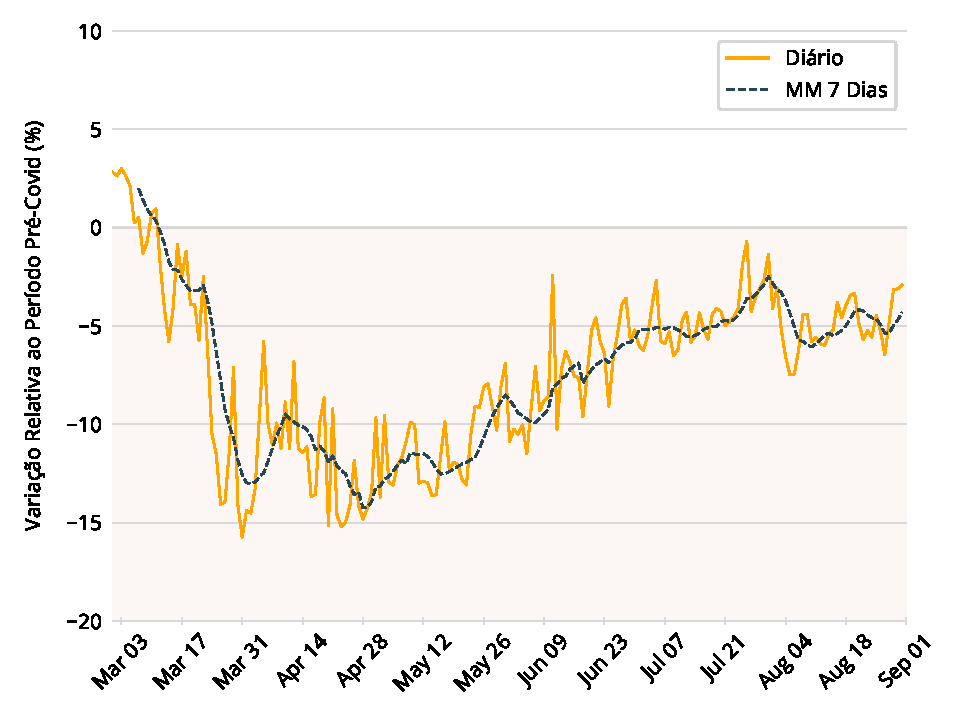
\includegraphics[width=\linewidth, keepaspectratio]{C:/Users/gabri/Desktop/electricity_rt/figures/results_2020_NE_notitle.pdf}
	\captionsetup{font={small}}
	\caption*{\textsuperscript{1} Valores normalizados para terem média zero entre 01 de janeiro e 29 de fevereiro de 2020. \\ \textsuperscript{2} Fontes: ONS e autor.}
\end{figure}

\begin{figure}[!htb]
	\centering
	\caption{Indicador de Consumo de Eletricidade -- Norte}
	\label{fig:figure3}
	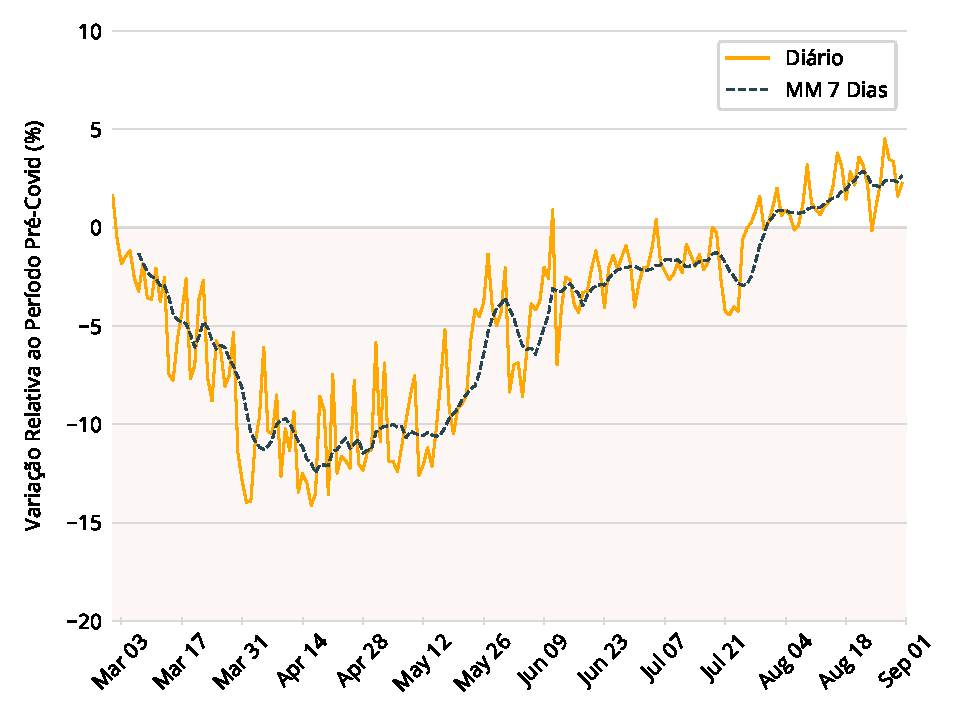
\includegraphics[width=\linewidth, keepaspectratio]{C:/Users/gabri/Desktop/electricity_rt/figures/results_2020_N_notitle.pdf}
	\captionsetup{font={small}}
	\caption*{\textsuperscript{1} Valores normalizados para terem média zero entre 01 de janeiro e 29 de fevereiro de 2020. \\ \textsuperscript{2} Fontes: ONS e autor.}
\end{figure}

\begin{figure}[!htb]
	\centering
	\caption{Indicador de Consumo de Eletricidade -- Sudeste/Centro-Oeste}
	\label{fig:figure4}
	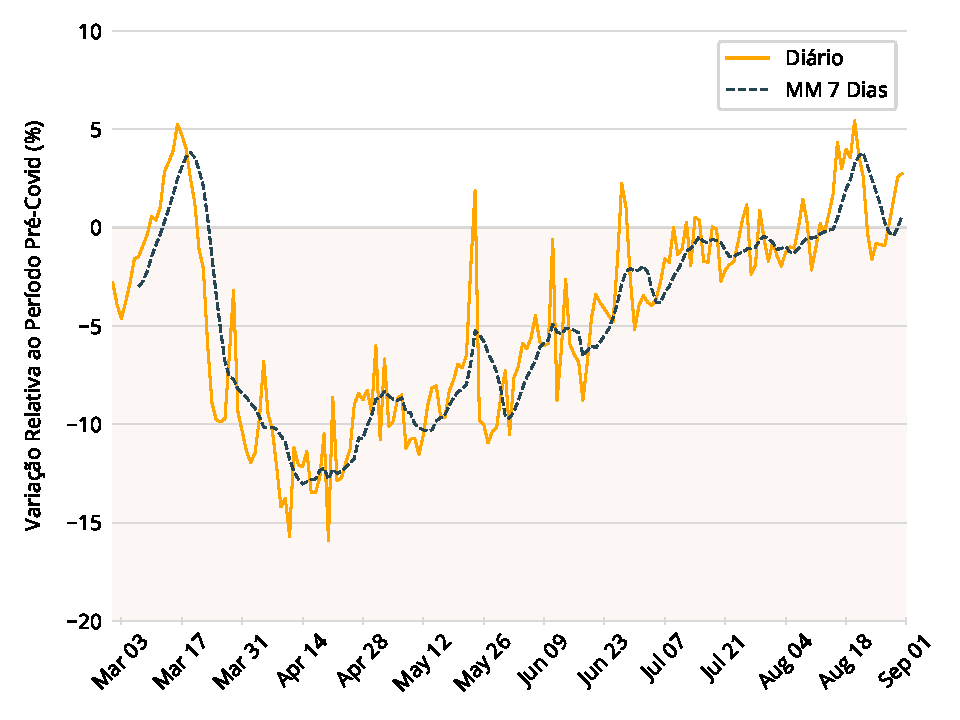
\includegraphics[width=\linewidth, keepaspectratio]{C:/Users/gabri/Desktop/electricity_rt/figures/results_2020_SE-CW_notitle.pdf}
	\captionsetup{font={small}}
	\caption*{\textsuperscript{1} Valores normalizados para terem média zero entre 01 de janeiro e 29 de fevereiro de 2020. \\ \textsuperscript{2} Fontes: ONS e autor.}
\end{figure}

\begin{figure}[!htb]
	\centering
	\caption{Indicador de Consumo de Eletricidade -- Sul}
	\label{fig:figure5}	
	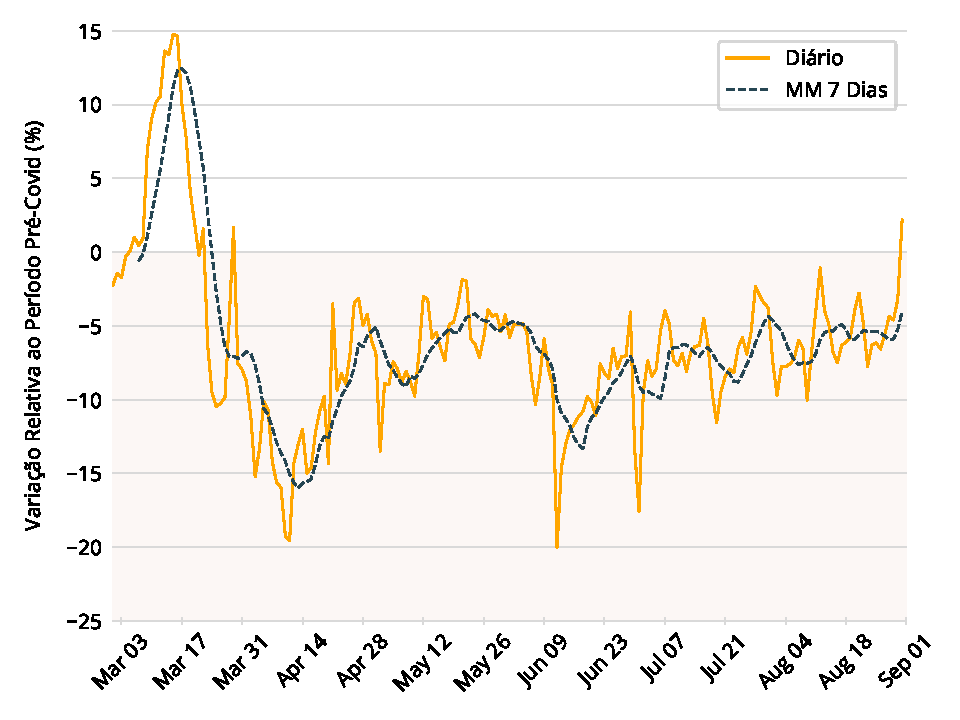
\includegraphics[width=\linewidth, keepaspectratio]{C:/Users/gabri/Desktop/electricity_rt/figures/results_2020_S_notitle.pdf}
	\captionsetup{font={small}}
	\caption*{\textsuperscript{1} Valores normalizados para terem média zero entre 01 de janeiro e 29 de fevereiro de 2020. \\ \textsuperscript{2} Fontes: ONS e autor.}
\end{figure}

\begin{figure}[!htbp]
	\centering
	\caption{Indicador de Consumo de Eletricidade -- Brasil}
	\label{fig:figure6}	
	\includegraphics[width=\linewidth, keepaspectratio]{C:/Users/gabri/Desktop/electricity_rt/figures/results_2020_Brazil_notitle.pdf}
	\captionsetup{font={small}}
	\caption*{\textsuperscript{1} Valores normalizados para terem média zero entre 01 de janeiro e 29 de fevereiro de 2020. \\ \textsuperscript{2} Fontes: ONS e autor.}
\end{figure}

\end{document}